\vspace{-0.09cm}
\section{Experimental Evaluation}
\vspace{-0.22cm}
\label{sec:calql_experiments}
The goal of our experimental evaluation is to study how well \methodname\ can facilitate sample-efficient online fine-tuning. To this end, we compare \methodname\ with several other state-of-the-art fine-tuning methods on a variety of offline RL benchmark tasks from D4RL~\cite{fu2020d4rl}, \citet{singh2020cog}, and \citet{nair2020accelerating}, evaluating performance before and after fine-tuning. We also study the effectiveness of \methodname\ on higher-dimensional tasks, where the policy and value function must process raw image observations. Finally, we perform empirical studies to understand the efficacy of \methodname\ with different dataset compositions and the impact of errors in the reference value function estimation.
% to understand the efficacy of \methodname\ with different dataset compositions 
% Finally, we perform several empirical studies to understand the efficacy of \methodname\ with different dataset compositions and to understand the impact of errors in reference function value estimation on \methodname.  

\begin{wrapfigure}{r}{0.48\linewidth}
\centering
\vspace{-0.6cm}
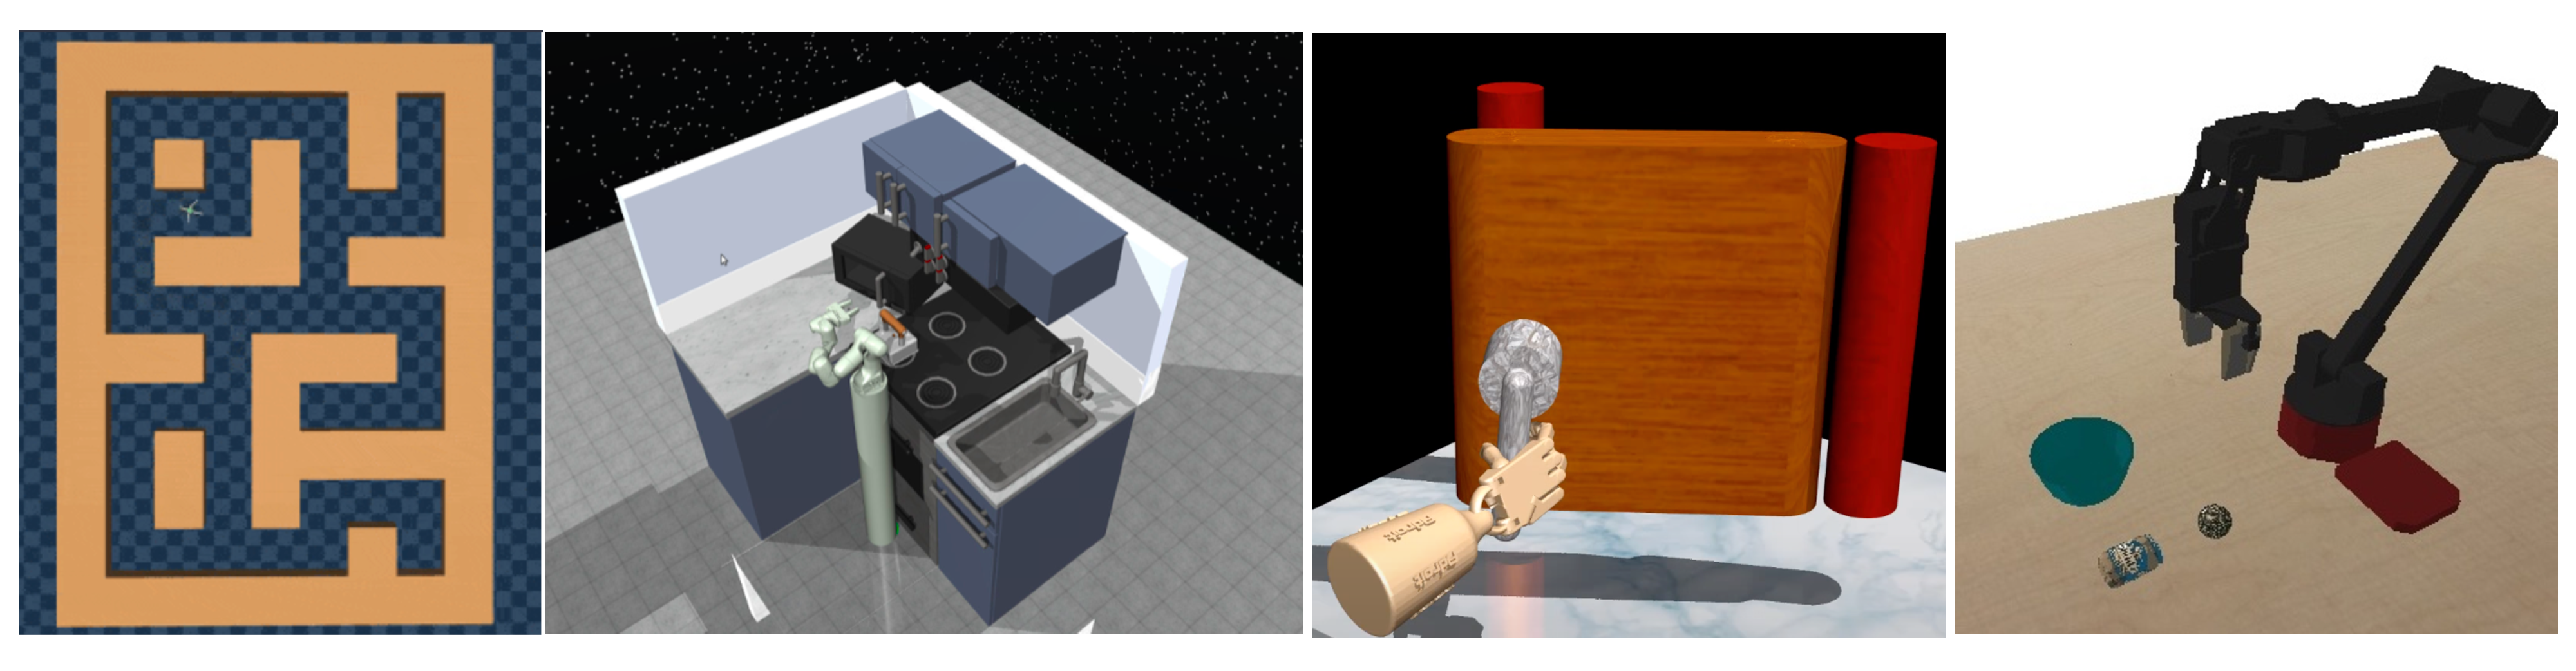
\includegraphics[width=0.97\linewidth]{chapters/cal_ql/figs-sample/envs_final.pdf}
\vspace{-0.4cm}
\caption{
\footnotesize{\textbf{Tasks:} We evaluate \methodname\ on a diverse set of benchmarks: \texttt{AntMaze} \& \texttt{Frankakitchen} domains from \cite{fu2020d4rl}, \texttt{Adroit} tasks from \cite{nair2020accelerating} and a vision-based robotic manipulation task from \cite{kumar2022pre}.}}
\label{fig:envs}
\vspace{-0.6cm}
\end{wrapfigure}
%%AK.5.6: Do we need this figure to be in the main paper given that we are tight on space?
\niparagraph{\textbf{Offline RL tasks and datasets.}} We evaluate \methodname\ on a number of benchmark tasks and datasets used by prior works~\cite{kostrikov2021iql,nair2020accelerating} to evaluate fine-tuning performance: \textbf{(1)} The {\texttt{AntMaze}} tasks from D4RL~\cite{fu2020d4rl} that require controlling an ant quadruped robot to navigate from a starting point to a desired goal location in a maze. The reward is +1 if the agent reaches within a pre-specified small radius around the goal and 0 otherwise. 
% We consider two kinds of maze layouts (medium and large mazes from \cite{fu2020d4rl}) and two data compositions: \textbf{play} and \textbf{diverse} that vary in coverage of actions at different regions of the state space and sub-optimality of the behavior policy. 
\textbf{(2)} The \texttt{FrankaKitchen} tasks from D4RL require controlling a 9-DoF Franka robot to attain a desired configuration of a kitchen. To succeed, a policy 
must complete four sub-tasks in the kitchen within a single rollout, and it receives a binary reward of +1/0 for every sub-task it completes. \textbf{(3)} Three \texttt{Adroit} dexterous manipulation tasks~\cite{rajeswaran2018dapg,kostrikov2021iql,nair2020accelerating} that require learning complex manipulation skills on a 28-DoF five-fingered hand to \textbf{(a)} manipulate a pen in-hand to a desired configuration (\texttt{pen-binary}), \textbf{(b)} open a door by unlatching the handle (\texttt{door-binary}), and \textbf{(c)} relocating a ball to a desired location (\texttt{relocate-binary}). The agent obtains a sparse binary +1/0 reward if it succeeds in solving the task. Each of these tasks only provides a narrow offline dataset consisting of 25 demonstrations collected via human teleoperation and additional trajectories collected by a BC policy.
Finally, to evaluate the efficacy of \methodname\ on a task where we learn from raw visual observations, we study \textbf{(4)} a pick-and-place task from prior work~\cite{singh2020cog,kumar2022pre} that requires learning to pick a ball and place it in a bowl, in the presence of distractors.

 
\iffalse

\textbf{Offline RL tasks and datasets.} We evaluate \methodname\ on a number of benchmark tasks and datasets used by prior works~\cite{kostrikov2021iql,nair2020accelerating} to evaluate fine-tuning performance: \textbf{(1)} The {\texttt{AntMaze}} tasks from D4RL~\cite{fu2020d4rl} that require controlling an 8-DoF ant quadruped robot to navigate from a starting point to a desired goal location in a maze. The reward is +1 if the agent reaches within a pre-specified small radius around the goal and 0 otherwise. We consider two kinds of maze layouts (medium and large mazes from \cite{fu2020d4rl}) and two data compositions: \textbf{play} and \textbf{diverse} that vary in coverage of actions at different regions of the state space and sub-optimality of the behavior policy. \textbf{(2)} The \texttt{FrankaKitchen} tasks from D4RL require controlling a 9-DoF Franka robot to attain a desired configuration of a kitchen. To succeed, a policy 
must complete four sub-tasks in the kitchen within a single rollout, and it receives a binary reward of +1/0 for every sub-task it completes. \textbf{(3)} Three \texttt{Adroit} dexterous manipulation tasks~\cite{rajeswaran2018dapg,kostrikov2021iql,nair2020accelerating} that require learning complex manipulation skills on a 28-DoF five-fingered hand to \textbf{(a)} manipulate a pen in-hand to a desired configuration (\texttt{pen-binary}), \textbf{(b)} open a door by unlatching the handle (\texttt{door-binary}), and \textbf{(c)} relocating a ball to a desired location (\texttt{relocate-binary}). An agent obtains a sparse binary +1/0 reward if it succeeds in solving the task. Each of these tasks only provides an extremely narrow offline dataset consisting of 25 demonstrations collected via human teleoperation and additional trajectories collected by a BC policy.
Finally, to evaluate the efficacy of \methodname\ on more challenging tasks where we must learn from raw visual observations, we study \textbf{(4)} a pick-and-place task from prior work~\cite{singh2020cog,kumar2022pre} that requires learning to pick a ball and place it in a bowl, in the presence of distractors.

\fi

\begin{figure}[t]
\begin{center}    
{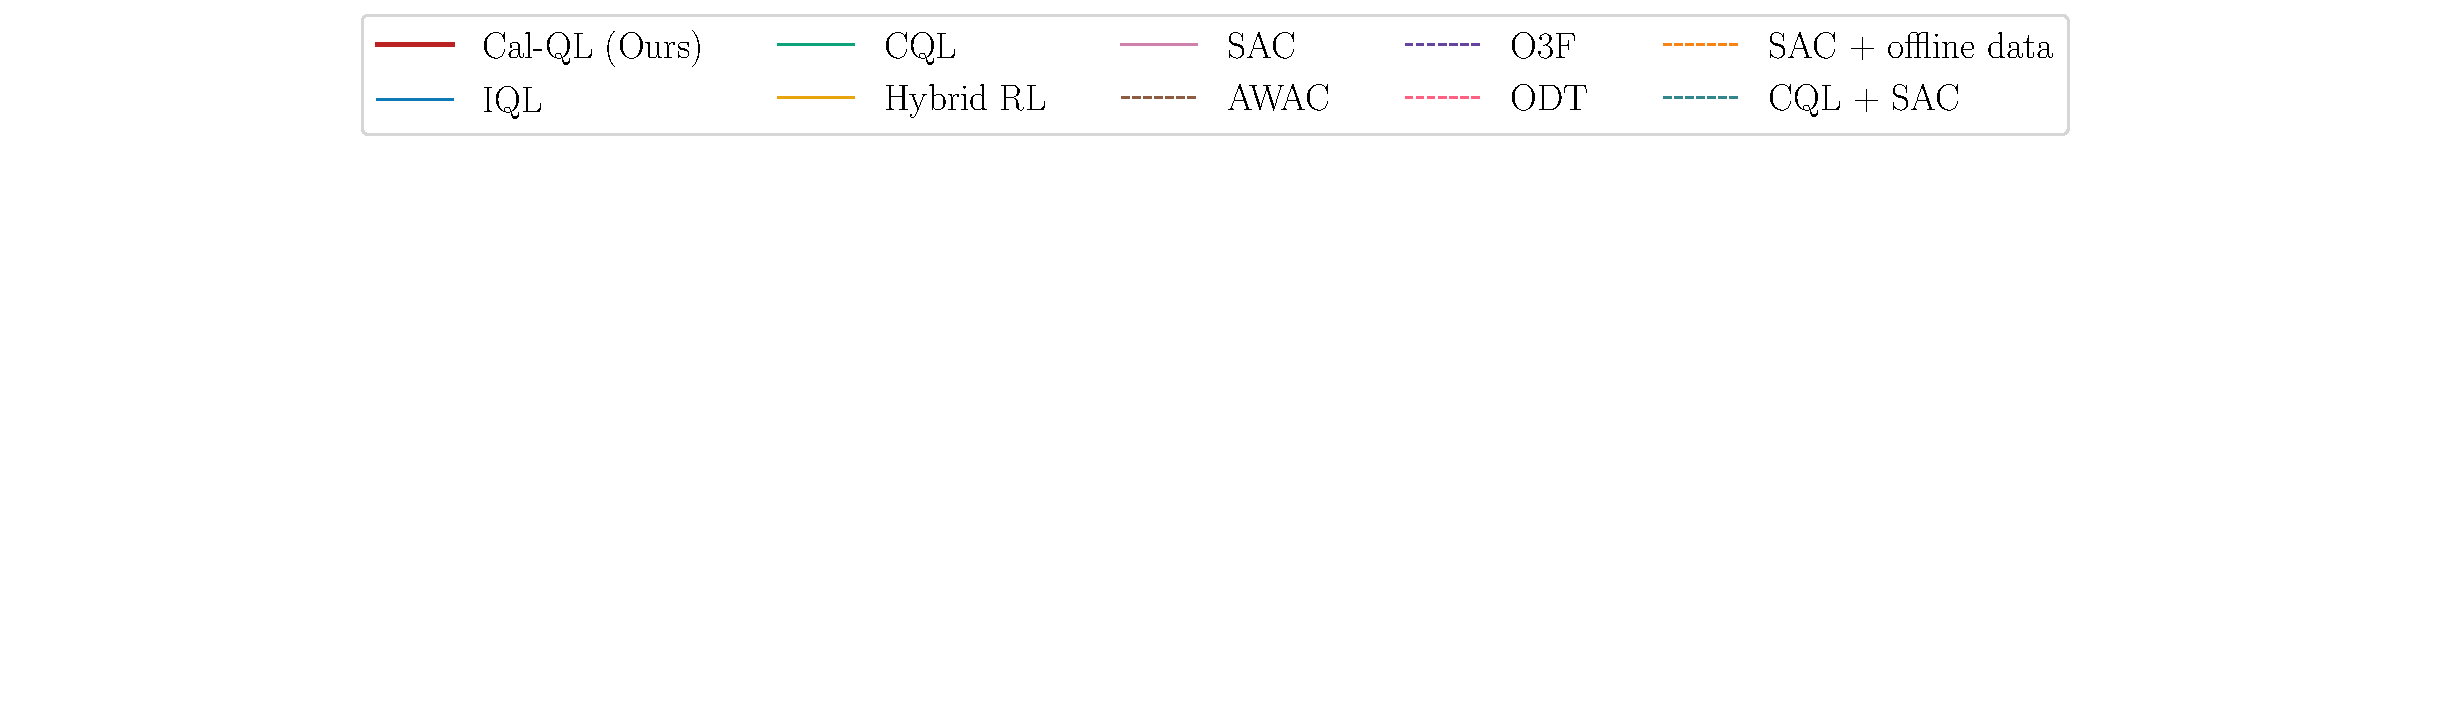
\includegraphics[clip,width=1\linewidth]{chapters/cal_ql/figs-sample/antmaze-final-caption.pdf}} 
{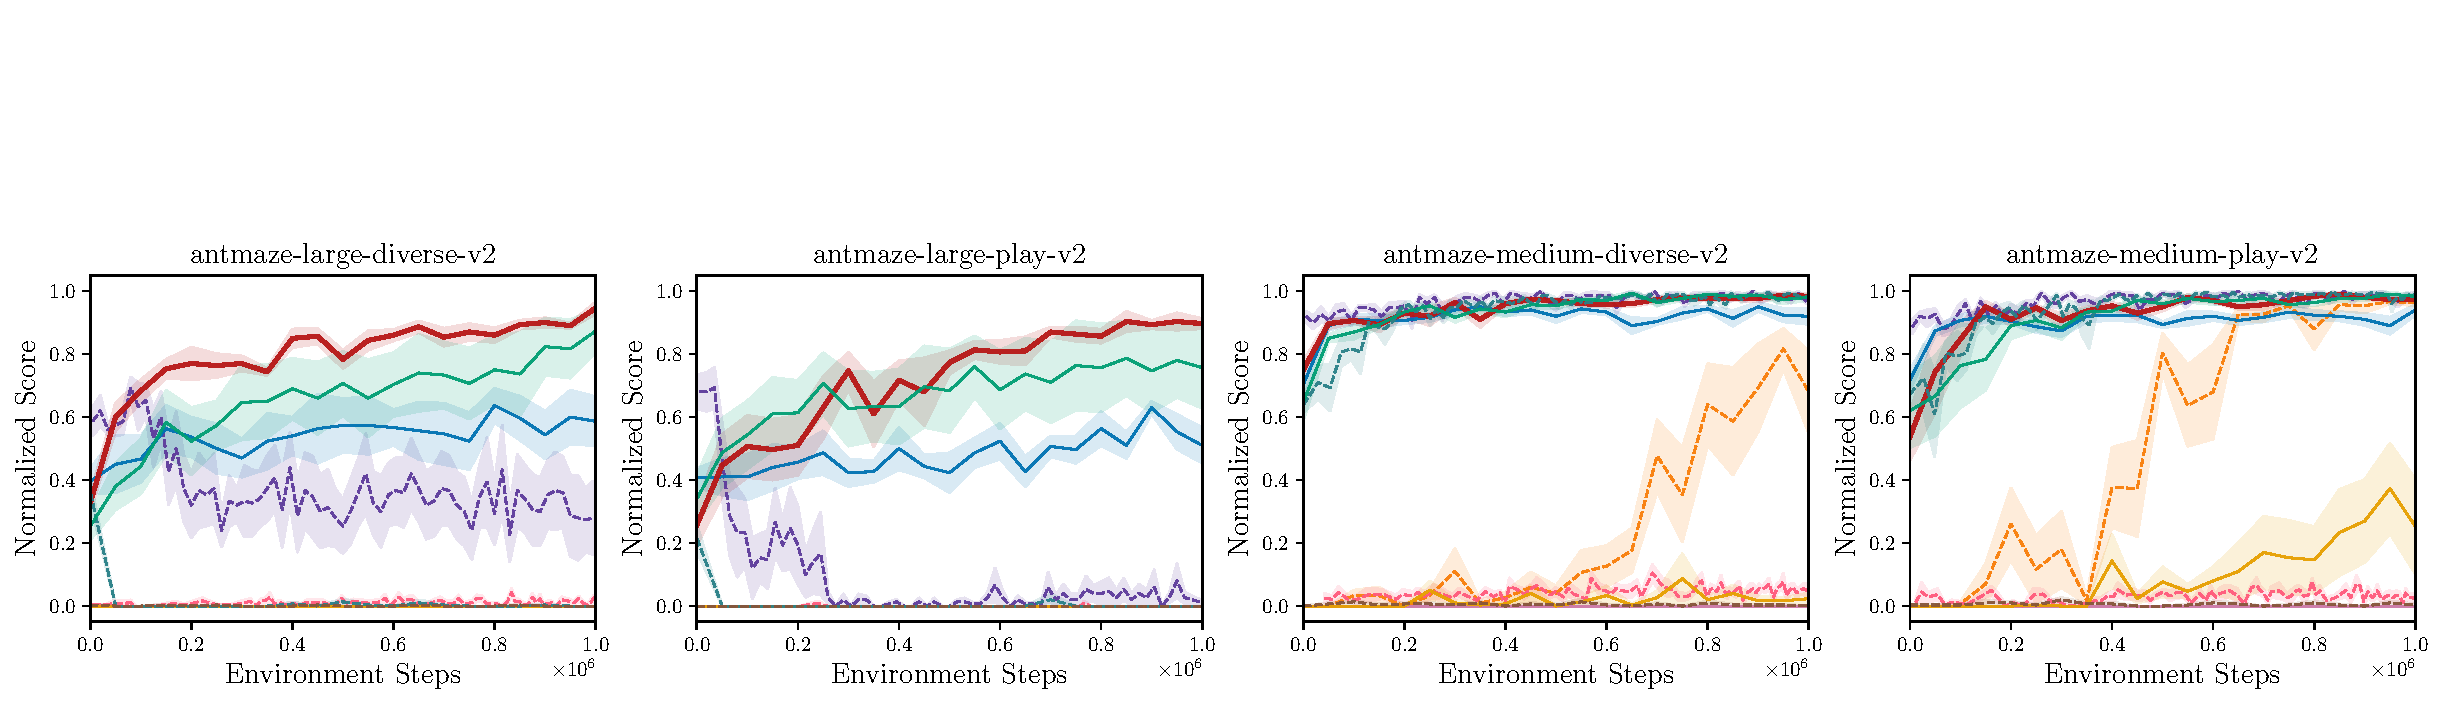
\includegraphics[clip,width=1\linewidth]{chapters/cal_ql/figs-sample/antmaze-final-plots-only.pdf}}\\{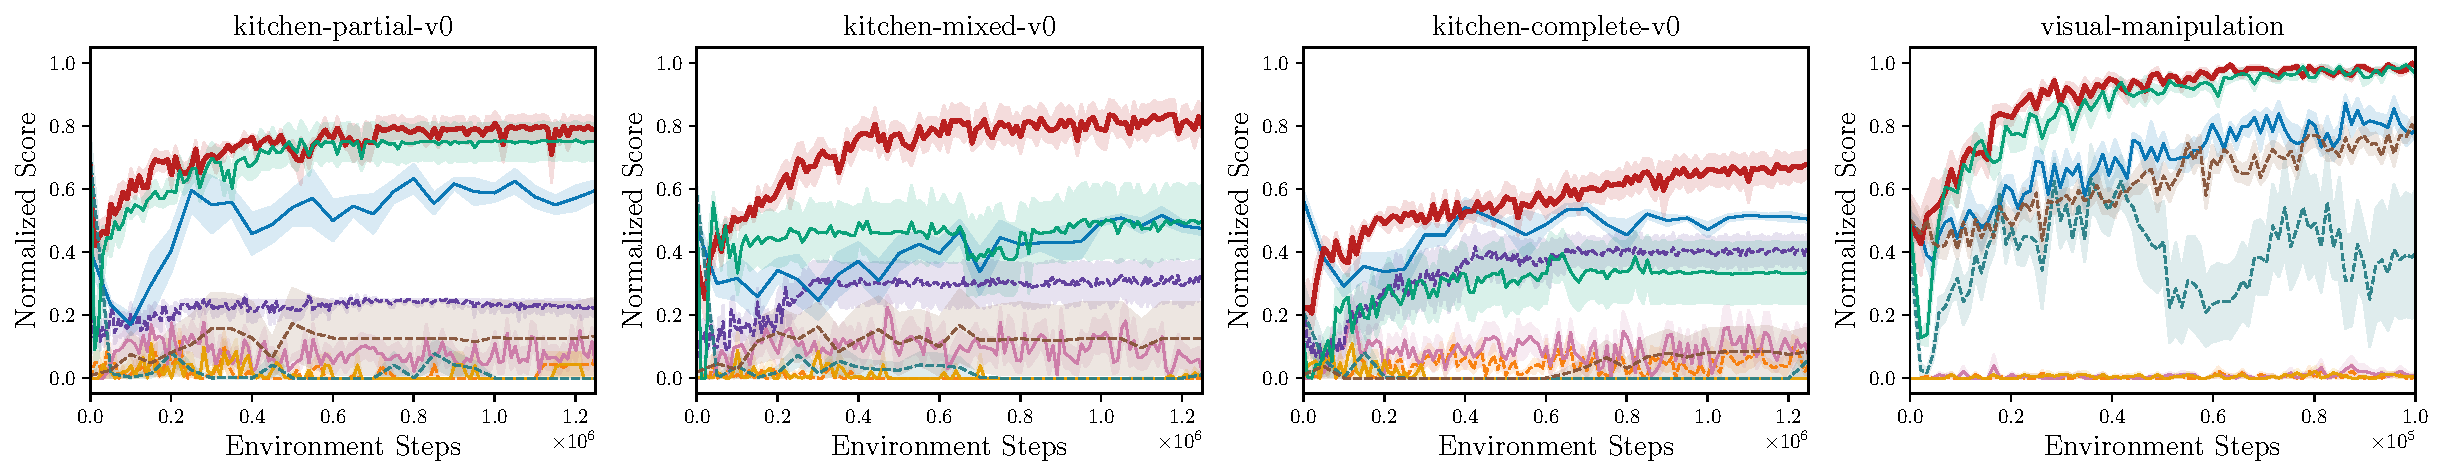
\includegraphics[clip,width=1\linewidth]{chapters/cal_ql/figs-sample/kitchen-cog-final.pdf}} {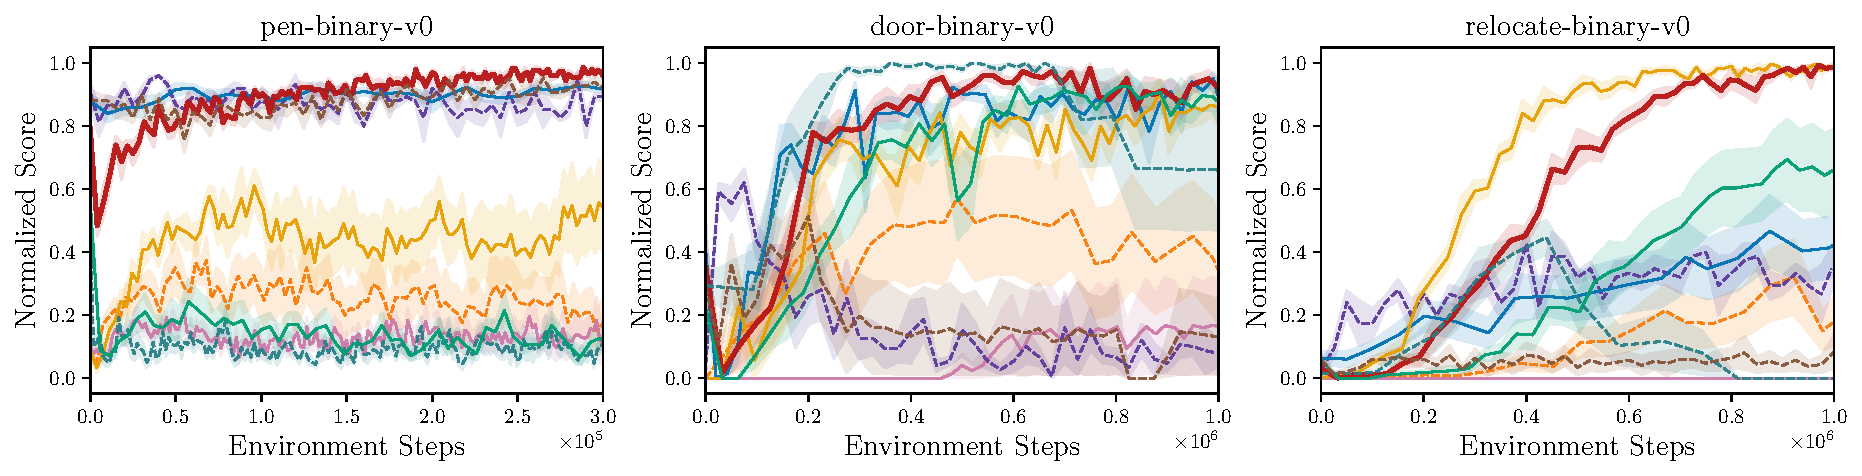
\includegraphics[clip,width=0.75\linewidth]{chapters/cal_ql/figs-sample/adroit-final.pdf}}
\end{center}
\vspace{-0.45cm}
\caption{\label{fig:all_tasks} \footnotesize{\textbf{Online fine-tuning after offline initialization on the benchmark tasks}. The plots show the online fine-tuning phase \emph{after} pre-training for each method (except SAC-based approaches which are not pre-trained). Observe that \methodname\ consistently matches or exceeds the speed and final performance of the best prior method and is the only algorithm to do so across all tasks. (6 seeds)}}
\vspace{-0.5cm}
\end{figure}


\noindent \textbf{Comparisons, prior methods, and evaluation protocol.} We compare \methodname\ to running online SAC~\cite{haarnoja2018soft} from scratch, as well as prior approaches that leverage offline data. This includes na\"ively fine-tuning offline RL methods such as CQL~\cite{kumar2020conservative} and IQL~\cite{kostrikov2021iql}, as well as fine-tuning with AWAC~\citep{nair2020accelerating}, O3F~\cite{mark2022fine} and online decision transformer (ODT)~\citep{zheng2022online}, methods specifically designed for offline RL followed by online fine-tuning. In addition, we also compare to a baseline that trains SAC~\cite{haarnoja2018soft} using both online data and offline data (denoted by ``SAC + offline data'') that mimics DDPGfD~\citep{vecerik2017leveraging} but utilizes SAC instead of DDPG. We also compare to Hybrid RL~\citep{song2023hybrid}, a recently proposed method that improves the sample efficiency of the ``SAC + offline data'' approach, and ``CQL+SAC'', which first pre-train with CQL and then run fine-tuning with SAC on a mixture of offline and online data without conservatism. More details of each method can be found in Appendix~\ref{app:calql_hyperparam}.
We present learning curves for online fine-tuning and also quantitatively evaluate each method on its ability to improve the initialization learned from offline data measured in terms of \textbf{(i)} final performance after a pre-defined number of steps per domain and \textbf{(ii)} the cumulative regret over the course of online fine-tuning. In Section~\ref{subsec:highutd}, we run \methodname\ with a higher update-to-data (UTD) ratio and compare it to RLPD~\cite{rlpd}, a more sample-efficient version of ``SAC + offline data''.

\vspace{-0.2cm}
\subsection{Empirical Results} 
\vspace{-0.2cm}

We first present a comparison of \methodname\ in terms of the normalized performance before and after fine-tuning in Table~\ref{tab:performance} and the cumulative regret in a fixed number of online steps in Table~\ref{tab:results_regret}. Following the protocol of \cite{fu2020d4rl}, we normalize the average return values for each domain with respect to the highest possible return (+4 in FrankaKitchen; +1 in other tasks; see Appendix~\ref{appendix:normalized_score} for more details).  

\textbf{\methodname\ improves the offline initialization significantly.} Observe in Table~\ref{tab:performance} and Figure~\ref{fig:all_tasks} that while the performance of offline initialization acquired by \methodname\ is comparable to that of other methods such as CQL and IQL, \methodname\ is able to improve over its offline initialization the most by \textbf{106.9\%} in aggregate and achieve the best fine-tuned performance in \textbf{9 out of 11} tasks.

\textbf{\methodname\ enables fast fine-tuning.} 
% To understand the efficacy of \methodname\ in enabling learning quickly during online fine-tuning, we measure the cumulative regret accumulated over the course of fine-tuning. 
Observe in Table~\ref{tab:results_regret} that \methodname\ achieves the smallest regret on \textbf{8 out of 11} tasks, attaining an average regret of 0.22 which improves over the next best method (IQL) by \textbf{42\%}. Intuitively, this means that \methodname\ does not require running highly sub-optimal policies. In tasks such as \texttt{relocate-binary}, \methodname\ enjoys the fast online learning benefits associated with na\"ive online RL methods that incorporate the offline data in the replay buffer (SAC + offline data and \methodname\ are the only two methods to  attain a score of $\geq$ 90\% on this task) unlike prior offline RL methods. As shown in Figure~\ref{fig:all_tasks}, in the \texttt{kitchen} and \texttt{antmaze} domains, \methodname\ brings the benefits of fast online learning together with a good offline initialization, improving drastically on the regret metric. Finally, observe that the initial unlearning at the beginning of fine-tuning with conservative methods observed in Section~\ref{sec:calql_empirical_analysis} is greatly alleviated in all tasks (see Appendix~\ref{app:cql_dip_zoom_in} for details).


\begin{table*}[h]
\scriptsize{
\begin{center}

\vspace{-0.1cm}
\!\!\!\!\resizebox{1.0\textwidth}{!}{
\begin{tabular}{l|c|c|c|c|c|c|c|c|c||c}
Task & CQL & IQL & AWAC & O3F & ODT & CQL+SAC & Hybrid SRL & SAC+od & SAC & Cal-QL (Ours) \\ \hline \hline
\texttt{large-diverse}  & 25 $\rightarrow$ 87 & 40 $\rightarrow$ 59 & 00 $\rightarrow$ 00 & 59 $\rightarrow$ 28 & 00 $\rightarrow$ 01 & 36 $\rightarrow$ 00 &  $\rightarrow$ 00 &  $\rightarrow$ 00 &  $\rightarrow$ 00 & 33 $\rightarrow$  \textbf{95} \\
\texttt{large-play}  & 34 $\rightarrow$ 76 & 41 $\rightarrow$ 51 & 00 $\rightarrow$ 00 & 68 $\rightarrow$ 01 & 00 $\rightarrow$ 00 & 21 $\rightarrow$ 00 &  $\rightarrow$ 00 &  $\rightarrow$ 00 &  $\rightarrow$ 00 & 26 $\rightarrow$  \textbf{90} \\
\texttt{medium-diverse}  & 65 $\rightarrow$  \textbf{98} & 70 $\rightarrow$ 92 & 00 $\rightarrow$ 00 & 92 $\rightarrow$ 97 & 00 $\rightarrow$ 03 & 64 $\rightarrow$ \textbf{98} &  $\rightarrow$ 02 &  $\rightarrow$ 68 &  $\rightarrow$ 00 & 75 $\rightarrow$ \textbf{98} \\
\texttt{medium-play}  & 62 $\rightarrow$ 98 & 72 $\rightarrow$ 94 & 00 $\rightarrow$ 00 & 89 $\rightarrow$ \textbf{99} & 00 $\rightarrow$ 05 & 67 $\rightarrow$ 98 &  $\rightarrow$ 25 &  $\rightarrow$ 96 &  $\rightarrow$ 00 & 54 $\rightarrow$ 97 \\  \hline
\texttt{partial}  & 71 $\rightarrow$ 75 & 40 $\rightarrow$ 60 & 01 $\rightarrow$ 13 & 11 $\rightarrow$ 22 & - & 71 $\rightarrow$ 00 &  $\rightarrow$ 00 &  $\rightarrow$ 07 &  $\rightarrow$ 03 & 67 $\rightarrow$ \textbf{79} \\
\texttt{mixed}  & 56 $\rightarrow$ 50 & 48 $\rightarrow$ 48 & 02 $\rightarrow$ 12 & 06 $\rightarrow$ 33 & - & 59 $\rightarrow$ 01 &   $\rightarrow$ 01 &   $\rightarrow$ 00 &   $\rightarrow$ 02 & 38 $\rightarrow$ \textbf{80} \\
\texttt{complete} & 13 $\rightarrow$ 34 & 57 $\rightarrow$ 50 & 01 $\rightarrow$ 08 & 17 $\rightarrow$ 41 & - & 21 $\rightarrow$ 06 &  $\rightarrow$ 00 & $\rightarrow$ 05 &  $\rightarrow$ 06 & 22 $\rightarrow$ \textbf{68} \\  \hline
\texttt{pen} & 55 $\rightarrow$ 13 & 88 $\rightarrow$ 92 & 88 $\rightarrow$ 92 & 91 $\rightarrow$ 89 & - & 48 $\rightarrow$ 10 &  $\rightarrow$ 54 &  $\rightarrow$ 17 &  $\rightarrow$ 11 & 79 $\rightarrow$ \textbf{99} \\
\texttt{door} & 22 $\rightarrow$ 88 & 41 $\rightarrow$ 88 & 29 $\rightarrow$ 13 & 04 $\rightarrow$ 08 & - & 29 $\rightarrow$ 66 &  $\rightarrow$ 88 &  $\rightarrow$ 39 &  $\rightarrow$ 17 & 35 $\rightarrow$ \textbf{92} \\
\texttt{relocate} & 06 $\rightarrow$ 69 & 06 $\rightarrow$ 45 & 06 $\rightarrow$ 08 & 03 $\rightarrow$ 35 & - & 01 $\rightarrow$ 00 &  $\rightarrow$ \textbf{99} &  $\rightarrow$ 16 &  $\rightarrow$ 00 & 03 $\rightarrow$ 98 \\  \hline
\texttt{manipulation} & 50 $\rightarrow$ 97 & 49 $\rightarrow$ 81 & 50 $\rightarrow$ 73 & - & - & 42 $\rightarrow$ 41 &  $\rightarrow$ 00 &  $\rightarrow$ 01 &  $\rightarrow$ 01 & 49 $\rightarrow$ \textbf{99} \\ \hline \hline
\textbf{average} & 42 $\rightarrow$ 71 & 50 $\rightarrow$ 69 & 16 $\rightarrow$ 20 & 44 $\rightarrow$ 45 & 00 $\rightarrow$ 02 & 42 $\rightarrow$ 29 &  $\rightarrow$ 24 &  $\rightarrow$ 23 &  $\rightarrow$ 04 & 44 $\rightarrow$ \textbf{90} \\ \hline
\textbf{improvement} & + 71.0\%  & + 37.7\%  & + 23.7\%  & + 3.0\%  & N/A  & - 30.3\%  & N/A &  N/A &  N/A & \textbf{+ 106.9\%}  \\
\end{tabular}}
\vspace{-0.15cm}
a\caption{\footnotesize{\textbf{Normalized score before \& after online fine-tuning.} Observe that \methodname\ improves over the best prior fine-tuning method and attains a much larger performance improvement over the course of online fine-tuning. The numbers represent the normalized score out of 100 following the convention in \citep{fu2020d4rl}.} \label{tab:performance}}
% \vspace{-0.1cm}
\end{center}
}
\end{table*}

% \begin{wraptable}{r}{0.66\linewidth}
\begin{table*}[h]
\vspace{-0.3cm}
\small{
\begin{center}
\resizebox{1.0\textwidth}{!}{
\begin{tabular}{l|c|c|c|c|c|c|c|c|c||c}
Task & CQL & IQL & AWAC & O3F & ODT & CQL+SAC & Hybrid RL & SAC+od & SAC & Cal-QL (Ours)\\ \hline \hline 
\texttt{large-diverse}  & 0.35 & 0.46 & 1.00 & 0.62 & 0.98 & 0.99 & 1.00 & 1.00 & 1.00 & \textbf{0.20}  \\
\texttt{large-play}     & 0.32 & 0.52 & 1.00 & 0.91 & 1.00 & 0.99 & 1.00 & 1.00 & 1.00 & \textbf{0.28}  \\
\texttt{medium-diverse} & 0.06 & 0.08 & 0.99 & \textbf{0.03} & 0.95 & 0.06 & 0.98 & 0.77 & 1.00 & 0.05  \\
\texttt{medium-play}    & 0.09 & 0.10 & 0.99 & \textbf{0.04} & 0.96 & 0.06 & 0.90 & 0.47 & 1.00 & 0.07  \\ \hline
\texttt{partial}                   & 0.31 & 0.49 & 0.89 & 0.78 & - & 0.97 & 0.98 & 0.98 & 0.92 & \textbf{0.27}  \\
\texttt{mixed}                     & 0.55 & 0.60 & 0.88 & 0.72 & - & 0.97 & 0.99 & 1.00 & 0.91 & \textbf{0.27}  \\
\texttt{complete}                  & 0.70 & 0.53 & 0.97 & 0.66 & - & 0.99 & 0.99 & 0.96 & 0.91 & \textbf{0.44}  \\ \hline
\texttt{pen}                       & 0.86 & \textbf{0.11} & 0.12 & 0.13 & - & 0.90 & 0.56 & 0.75 & 0.87 & \textbf{0.11}  \\
\texttt{door}                      & 0.36 & 0.25 & 0.81 & 0.82 & - & \textbf{0.23} & 0.35 & 0.60 & 0.94 & \textbf{0.23}  \\
\texttt{relocate}                  & 0.71 & 0.74 & 0.95 & 0.71 & - & 0.86 & \textbf{0.30} & 0.89 & 1.00 & 0.43  \\ \hline
\texttt{manipulation}              & 0.15 & 0.32 & 0.38 & - & - & 0.61 & 1.00 & 1.00 & 0.99 & \textbf{0.11}   \\ \hline \hline
\textbf{average}              & 0.41 & 0.38 & 0.82 & 0.54 & 0.97 & 0.69 & 0.82 & 0.86 & 0.96 & \textbf{0.22} 

\end{tabular}}
\vspace{-0.05cm}
\caption{\footnotesize{\textbf{Cumulative regret averaged over the steps of fine-tuning.} The smaller the better and 1.00 is the worst. \methodname\ attains the smallest overall regret, achieving the best performance among 8 / 11 tasks.}}
\label{tab:results_regret}

\vspace{-0.6cm}
\end{center}}
% \end{wraptable}
\end{table*}

\vspace{-0.1cm}
\subsection{\methodname\ With High Update-to-Data (UTD) Ratio}
\label{subsec:highutd}
\vspace{-0.2cm}


We can further enhance the online sample efficiency of \methodname\ by increasing the number of gradient steps per environment step made by the algorithm. The number of updates per environment step is usually called the update-to-data (UTD) ratio.
% In Figure~\ref{fig:utd-cog}, we present the performance of \methodname\ with $\text{UTD}=5$ on the \texttt{visual-manipulation} task. We can see that \methodname\ can achieve higher sample efficiency by using $\text{UTD}=5$, and the initial unlearning disappears completely which we studied previously in Section~\ref{sec:empirical_analysis}. Interestingly, while prior fine-tuning methods such as IQL do not improve with a higher UTD (see Figure~\ref{fig:utd-cog}), \methodname\ and CQL benefit from using a higher UTD ratio. We will further discuss this in Appendix~\ref{appendix:more_discussion_on_finetuning}.
In standard online RL, running off-policy Q-learning with a high UTD value (e.g., 20, compared to the typical value of 1) often results in challenges pertaining to overfitting~\citep{li2023efficient, redq, rlpd, replaybarrier}. As expected, we noticed that running \methodname\ with a high UTD value also leads these overfitting challenges. To address these challenges in high UTD settings, we combine \methodname\ with the Q-function architecture in recent work, RLPD~\citep{rlpd} (i.e., we utilized layer normalization in the Q-function and ensembles akin to \citep{redq}), that attempts to tackle overfitting challenges. Note that \methodname\ still first pre-trains on the offline dataset using Equation~\ref{eqn:cal_ql_training} followed by online fine-tuning, unlike RLPD that runs online RL right from the start.
In Figure~\ref{fig:rlpd}, we compare \methodname\ ($\text{UTD}=20$) with RLPD~\cite{rlpd} ($\text{UTD}=20$) and also \methodname\ ($\text{UTD}=1$) as a baseline. Observe that \methodname\ ($\text{UTD}=20$) improves over \methodname\ ($\text{UTD}=1$) and training from scratch (RLPD).   

\iffalse
%%AK: This is the original version of this section

We can further enhance the online sample efficiency of \methodname\ by increasing the number of gradient steps per environment step made by the algorithm. The number of updates per environment step is usually called the update-to-data (UTD) ratio. We will now evaluate \methodname\ with a high UTD ratio. In Figure~\ref{fig:utd-cog}, we present the performance of \methodname\ with $\text{UTD}=5$ on the \texttt{visual-manipulation} task. We can see that \methodname\ can achieve higher sample efficiency by using $\text{UTD}=5$, and the initial unlearning disappears completely which we studied previously in Section~\ref{sec:empirical_analysis}. Interestingly, while prior fine-tuning methods such as IQL do not improve with a higher UTD (see Figure~\ref{fig:utd-cog}), \methodname\ and CQL benefit from using a higher UTD ratio. We will further discuss this in Appendix~\ref{appendix:more_discussion_on_finetuning}.

We noticed that simply running \methodname\ with an even higher UTD value (e.g., 20) leads to previously-observed challenges pertaining to overfitting~\citep{li2023efficient, redq, rlpd, replaybarrier}. To address these challenges in high UTD settings, we ran \methodname\ in conjunction with the Q-function architecture in \cite{rlpd} (i.e., we utilized layer normalization in the Q-function and ensembles akin to \cite{redq}) to prevent overfitting. Note that \methodname\ still first pre-trains on the offline dataset using Equation~\ref{eqn:cal_ql_training} followed by online fine-tuning, unlike RLPD that runs online RL from scratch on offline and online data. 
In Figure~\ref{fig:rlpd}, we compare \methodname\ ($\text{UTD}=20$) with RLPD~\cite{rlpd} ($\text{UTD}=20$) and also \methodname\ ($\text{UTD}=1$) as a baseline. Observe that \methodname\ ($\text{UTD}=20$) improves over \methodname\ ($\text{UTD}=1$) and training from scratch (RLPD).   

\begin{figure}[ht]
\vspace{-0.3cm}
\begin{center}
\centerline{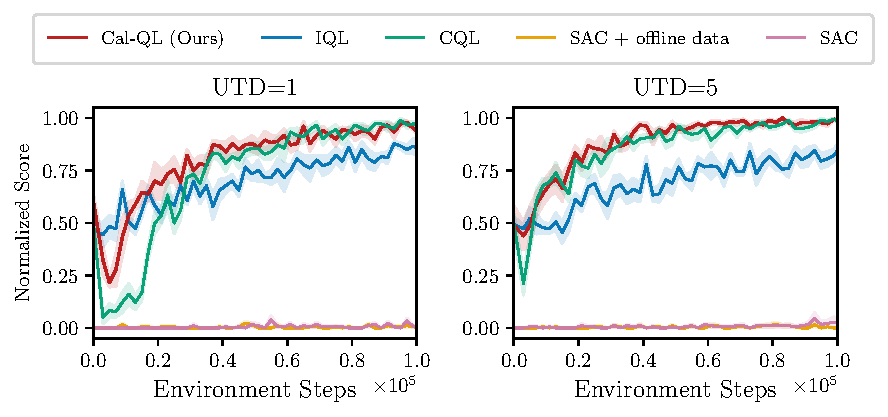
\includegraphics[width=0.55\textwidth]{chapters/cal_ql/figs-sample/cog-highutd-final.pdf}}
\vspace{-0.3cm}
\caption{\label{fig:utd-cog}\footnotesize{\textbf{UTD ablation}: We observe that using a higher UTD ratio can lead to higher sample efficiency for \methodname\ and CQL but not for IQL.}}
\end{center}
\vspace{-0.9cm}
\end{figure}

\fi

\begin{figure}[h]
\begin{center}    
{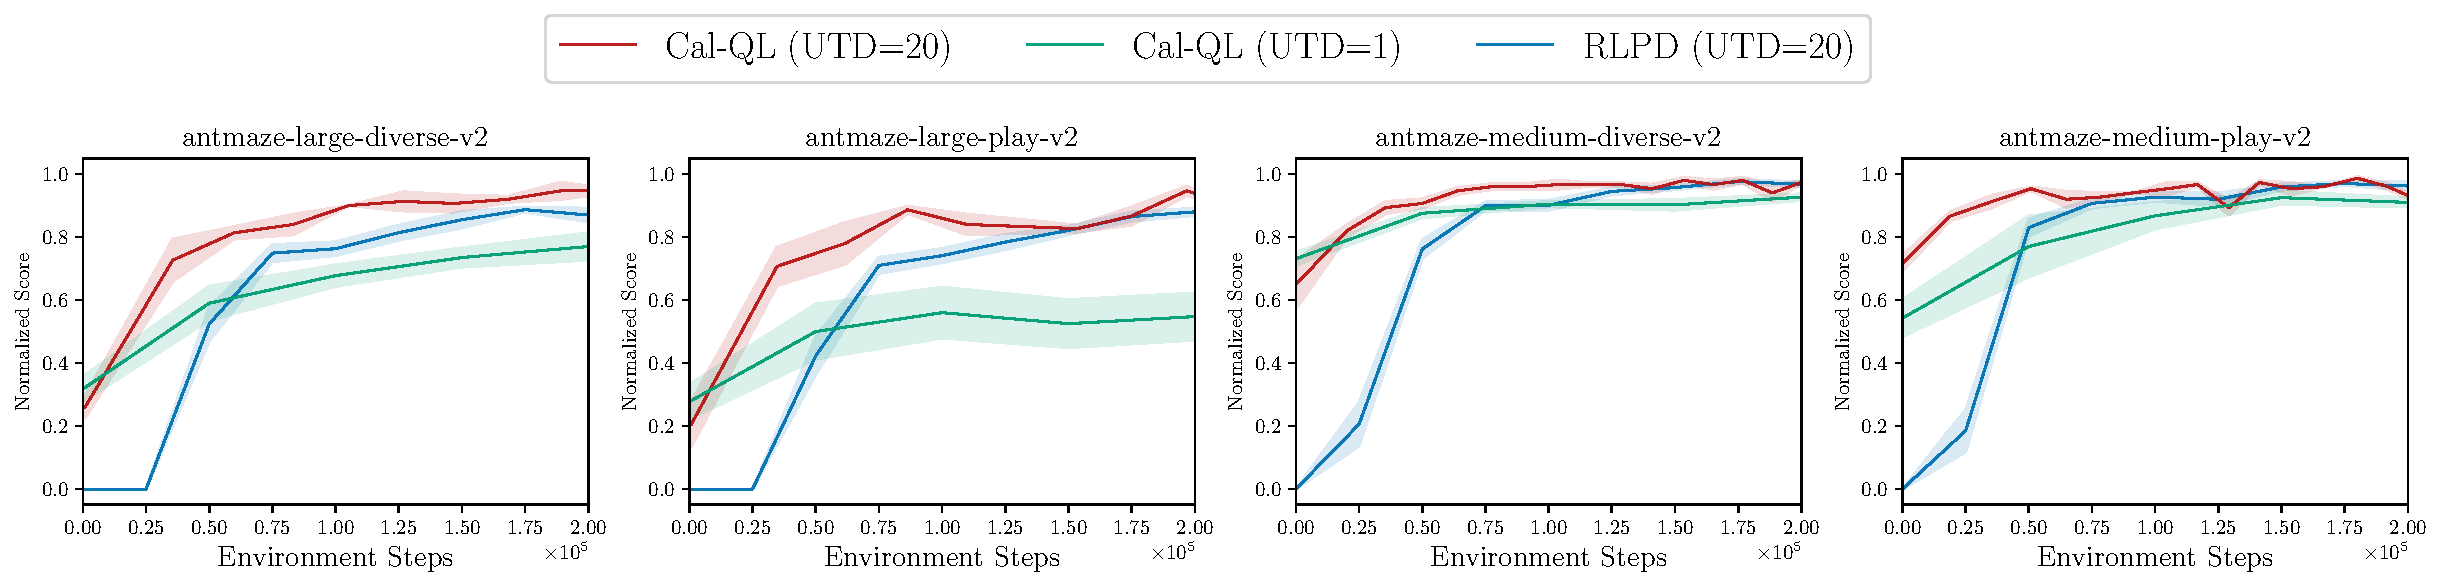
\includegraphics[clip,width=1\linewidth]{chapters/cal_ql/figs-sample/antmaze-utd20-rlpd-final.pdf}} {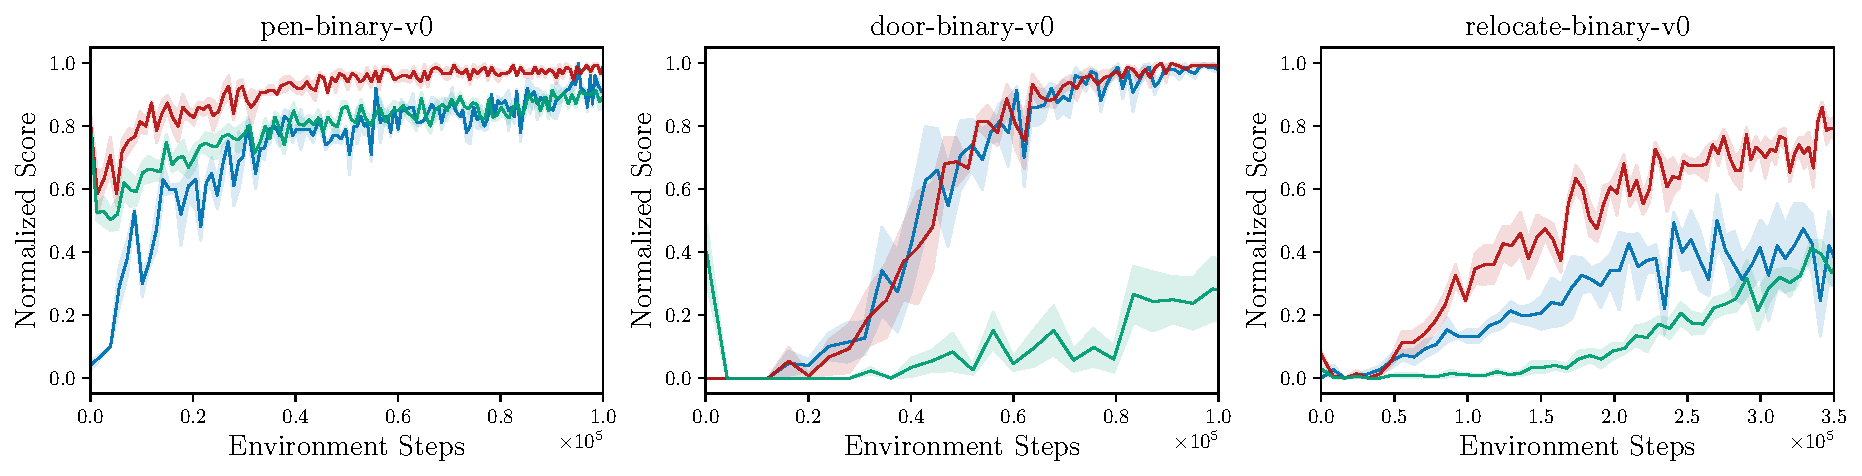
\includegraphics[clip,width=0.75\linewidth]{chapters/cal_ql/figs-sample/adroit-rlpd-final.pdf}}
\end{center}
\vspace{-0.3cm}
\caption{\label{fig:rlpd} \footnotesize{\textbf{\methodname\ with UTD=20}. Incorporating design choices from RLPD enables \methodname\ to achieve sample-efficient fine-tuning with UTD=20. Specifically, \methodname\ generally attains similar or higher asymptotic performance as RLPD, while also exhibiting a smaller cumulative regret.}}
\vspace{-0.6cm}
\end{figure}





\vspace{-0.2cm}
\subsection{Understanding the Behavior of \methodname}
\label{subsec:diagonistic}
\vspace{-0.3cm}

In this section, we aim to understand the behavior of \methodname\ by performing controlled experiments that modify the dataset composition, and by investigating various metrics to understand the properties of scenarios where utilizing \methodname\ is especially important for online fine-tuning.         

\textbf{Effect of data composition.} To understand the efficacy of \methodname\ with different data compositions, we ran it on a newly constructed fine-tuning task on the medium-size \texttt{AntMaze} domain with a low-coverage offline dataset, which is generated via a scripted controller that starts from a fixed initial position and navigates the ant to a fixed goal position. In Figure~\ref{fig:ant-narrow}, we plot the performance of \methodname\ and baseline CQL (for comparison) on this task, alongside the trend of average Q-values over the course of offline pre-training (to the left of the dashed vertical line, before 250 training epochs) and online fine-tuning (to the right of the vertical dashed line, after 250 training epochs), and the trend of \emph{bounding rate}, i.e., the fraction of transitions in the data-buffer for which the constraint in \methodname\ actively lower-bounds the learned Q-function with the reference value. For comparison, we also plot these quantities for a diverse dataset with high coverage on the task (we use the \texttt{antmaze-medium-diverse} from \cite{fu2020d4rl} as a representative diverse dataset) in Figure~\ref{fig:ant-narrow}. 

Observe that for the diverse dataset, both na\"ive CQL and \methodname\ perform similarly, and indeed, the learned Q-values behave similarly for both of these methods. In this setting, online learning doesn't spend samples to correct the Q-function when fine-tuning begins leading to a low bounding rate, almost always close to 0. Instead, with the narrow dataset, we observe that the Q-values learned by na\"ive CQL are much smaller, and are corrected once fine-tuning begins. This correction co-occurs with a drop in performance (solid blue line on left), and na\"ive CQL is unable to recover from this drop. \methodname\, which calibrates the scale of the Q-function for many more samples in the dataset, stably transitions to online fine-tuning with no unlearning (solid red line on left). 

\begin{wrapfigure}{r}{0.54\textwidth}
\vspace{-0.35cm}
\centering
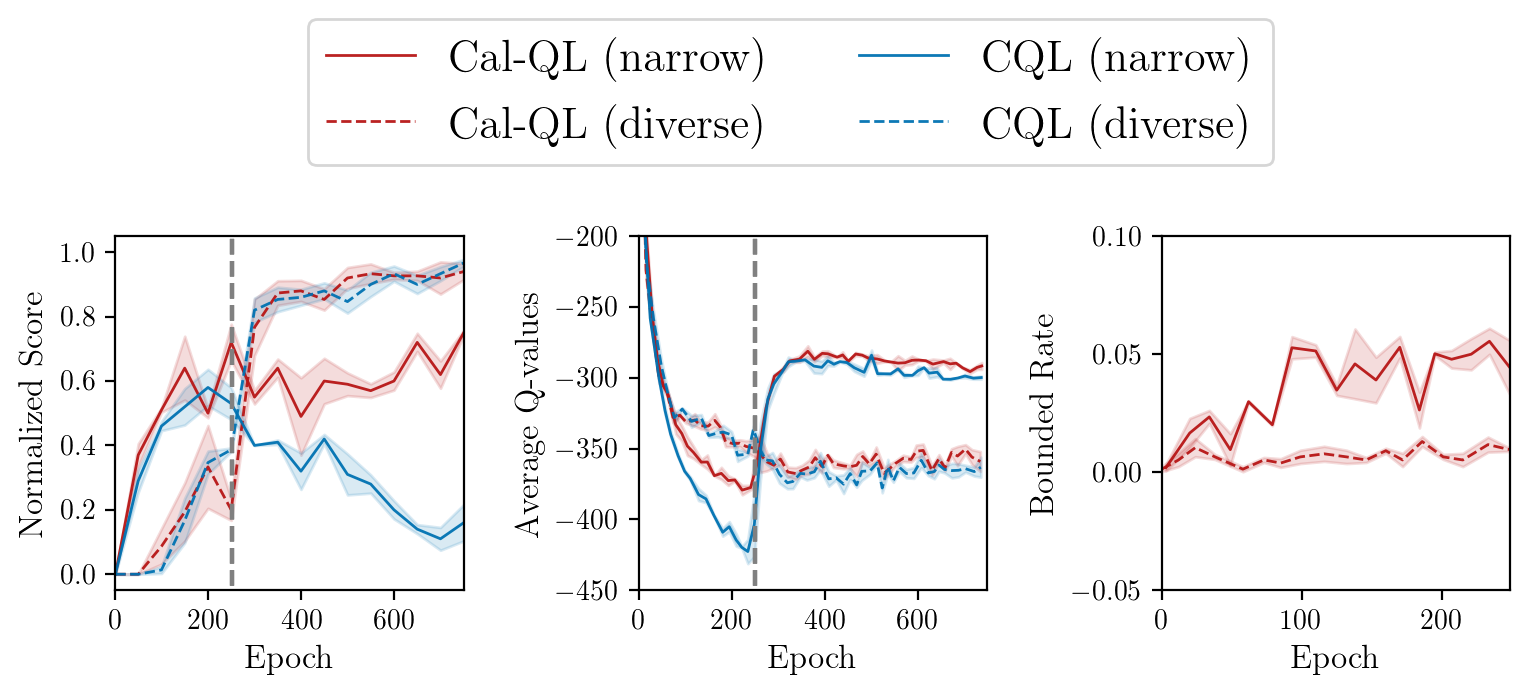
\includegraphics[width=0.97\linewidth]{chapters/cal_ql/figs-sample/diagnose-1.png}
\vspace{-0.3cm}
\caption{
\footnotesize{\textbf{Performance of \methodname\ with data compositions.} \methodname\ is most effective with narrow datasets, where Q-values need to be corrected at the beginning of fine-tuning.}
}
\label{fig:ant-narrow}
\vspace{-0.35cm}
\end{wrapfigure}


This suggests that in settings with narrow datasets (e.g., in the experiment above and in the \texttt{adroit} and \texttt{visual-manipulation} domains from Figure~\ref{fig:all_tasks}), Q-values learned by na\"ive conservative methods are more likely to be smaller than the ground-truth Q-function of the behavior policy due to function approximation errors. Hence utilizing \methodname\ to calibrate the Q-function against the behavior policy can be significantly helpful. On the other hand, with significantly high-coverage datasets, especially in problems where the behavior policy is also random and sub-optimal, Q-values learned by na\"ive methods are likely to already be calibrated with respect to those of the behavior policy. Therefore no explicit calibration might be needed (and indeed, the bounding rate tends to be very close to 0 as shown in Figure~\ref{fig:ant-narrow}). In this case, \methodname\ will revert back to standard CQL, as we observe in the case of the diverse dataset above. This intuition is also reflected in Theorem~\ref{thm:main-thm-informal}: when the reference policy $\mu$ is close to a narrow, expert policy, we would expect \methodname\ to be especially effective in controlling the efficiency of online fine-tuning. {We also present a diagnostic study of \methodname\ when the reference value function is estimated by fitting a neural network in Appendix~\ref{app:nn_value_function}}, and find that estimation errors in this model of the reference function do not affect performance significantly. 




\vspace{-0.2cm}